% =====================================================================================================
% Paper draft (first draft for advisor discussion)
% Built from the XRB-pilot repository at commit 666c2e0ad6c490a5014d4290f3becc571e07132d.
% No analysis was re-run for this draft; every number is read from committed result files
% (see paper_draft/claim_evidence.csv for the claim -> file -> row mapping).
% Compile:  latexmk -pdf main.tex   (or pdflatex, bibtex, pdflatex, pdflatex)
% =====================================================================================================
\documentclass[11pt,a4paper]{article}
\usepackage[T1]{fontenc}
\usepackage[utf8]{inputenc}
\usepackage{lmodern}
\usepackage[margin=2.4cm]{geometry}
\usepackage{amsmath,amssymb}
\usepackage{graphicx}
\usepackage{booktabs,tabularx,multirow,threeparttable}
\usepackage[table]{xcolor}
\usepackage{tikz}
\usetikzlibrary{positioning,arrows.meta,fit,calc}
\usepackage[round,authoryear]{natbib}
\usepackage{microtype}
\usepackage[font=small,labelfont=bf]{caption}
\usepackage{lineno}
\usepackage{setspace}
\usepackage[colorlinks=true,linkcolor=blue!50!black,citecolor=blue!50!black,urlcolor=blue!50!black]{hyperref}
\usepackage[capitalise,noabbrev]{cleveref}
\setstretch{1.1}
\setlength{\emergencystretch}{3em}
\linenumbers
\renewcommand{\linenumberfont}{\normalfont\tiny\sffamily\color{gray}}

% ---- macros ----
\newcommand{\placeholder}[1]{\textcolor{red}{\textbf{[#1]}}}
\newcommand{\ci}[2]{$[#1,\,#2]$}
\newcommand{\Hcol}{\textsf{H}}
\newcommand{\HT}{\textsf{H+T}}
\newcommand{\nuc}{\nu_{\rm c}}
\newcommand{\dAUC}{\Delta\mathrm{AUC}}

\title{What do X-ray colours capture, and what does low-frequency variability add?\\[2pt]
\large Black hole versus neutron star classification of X-ray binaries excluded from training,\\ with RXTE and NICER}
\author{\placeholder{Author names and order to be decided}\\[2pt]
\small\placeholder{Affiliations to be added}\\
\small\placeholder{Corresponding author e-mail}}
\date{First draft for advisor discussion --- \today\\
\small Repository state: \texttt{Chipwwwwww/XRB-pilot} commit \texttt{666c2e0}; technical report \texttt{report\_en/main.pdf} (205 pp., same commit)}

\begin{document}
\maketitle

% -----------------------------------------------------------------------------------------------------
\begin{abstract}
\noindent
Classifiers that assign a black hole (BH) or neutron star (NS) to an X-ray binary from a single observation are usually
summarised by one accuracy, which mixes three questions: which part of the data carries the signal, in which accretion
states, and whether it holds for unseen sources. We address them with evaluations in which every test source is excluded
from training, using RXTE/PCA and NICER/XTI observations of dynamically confirmed BHs and of bursting or pulsating NSs.
For 31 RXTE sources (7~BHs, 456~observations), a logistic regression on two hardness ratios reached a source-level area
under the ROC curve (AUC) of 0.923 (95\% source-bootstrap interval 0.804--0.994). The full 5--25~keV spectrum, extra
energy bands, 17 times more observations and a nested search over eight algorithms added no detectable improvement,
which does not demonstrate equivalence. The colour-only observation-level AUC was 0.954 in observations with weak
0.1--4~Hz variability (``soft-like'') but 0.646 in observations with strong variability (``hard-like''). Within hard-like
observations, adding fractional rms in three bands between 0.016 and 4~Hz raised the observation-level AUC in RXTE
($+0.264$ \ci{+0.048}{+0.455}) and, with a random forest, in each NICER set. On 198 previously unanalysed NICER
observations, processed with a frozen pipeline that included 3C50 background correction and classified with a random
forest specified before download, the hard-like AUC rose from 0.680 to 0.864 ($+0.184$ \ci{+0.049}{+0.337}; 74
observations of 8~BHs and 19~NSs); the source-level gain was $+0.125$ \ci{-0.053}{+0.303}. These observations come from
sources already in the sample, the analysis plans were written after earlier results, and only 16 confirmed BHs had
usable timing data, so confirmation on new sources is still required. A lower characteristic variability frequency of
BHs at matched colour appeared in every NICER set, but its significance depended on the background treatment.
\end{abstract}

\noindent\textbf{Keywords:} X-rays: binaries --- accretion --- stars: black holes --- stars: neutron --- methods: statistical
\placeholder{journal keyword list to be matched to the target journal}

% =====================================================================================================
\section{Introduction}\label{sec:intro}

The nature of the compact object in an X-ray binary is established securely in only two ways. A dynamical mass above the
maximum NS mass, usually measured from optical or infrared spectroscopy of the donor star in quiescence, identifies a
BH \citep{CorralSantana2016,Marcel2026}. Thermonuclear (type~I) X-ray bursts or coherent pulsations identify an NS
\citep{Galloway2008,Galloway2020}. Many X-ray binaries, including most newly discovered transients during their first
outburst, have neither. In practice the compact object is often inferred from X-ray phenomenology: the shape of the
spectrum, its evolution through accretion states, and the variability
\citep{RemillardMcClintock2006}.

\paragraph{What is known physically.}
An NS has a surface, whereas a BH has an event horizon. Emission from the NS surface or boundary layer changes the X-ray
spectrum most clearly when the source is bright and soft. \citet{DoneGierlinski2003} compared RXTE colour--colour diagrams
of atoll sources and BH binaries and attributed the systematic differences between their tracks to the presence of an NS
surface. In the hard state, BH and NS spectra are more alike in the 2--20~keV range. \citet{Burke2017} found that their
differences lie mainly in Comptonization parameters (electron temperature and Compton $y$), which require broad-band
spectral fitting. Variability has long been used as a discriminant. \citet{SunyaevRevnivtsev2000} proposed that significant
power above a few hundred Hz in the low/hard state indicates an NS. At lower frequencies, broad-band noise and
quasi-periodic features follow similar frequency correlations in BH and low-luminosity NS systems
\citep{WijnandsvanderKlis1999}. However, the highest characteristic frequencies of BHs lie several times below those of
NSs \citep{KleinWolt2008}. Power colours show that NS low-mass X-ray binaries move through tracks that closely resemble
those of BHs \citep{Heil2015,GardenierUttley2018}. Low-frequency variability is therefore known to be similar in BHs and
NSs in many respects. It is not obvious whether it contains information that complements the spectral colours.

\paragraph{What machine-learning studies have done.}
\citet{Pattnaik2021} trained a random forest on RXTE/PCA 5--25~keV spectra of 61 low-mass X-ray binaries (about 15\,000
observations). They evaluated it with whole sources held out of training and reported an average accuracy of
$87\pm13$~per~cent. They also noted that misclassifications are more frequent in hard and intermediate states and at low
signal-to-noise ratio. \citet{deBeurs2022} compared Gaussian-process, $k$-nearest-neighbour and support-vector classifiers
on MAXI colour--colour--intensity diagrams, separating BHs, non-pulsing NSs and pulsars, again with sources held out.
\citet{Garg2026} trained neural networks on the RXTE spectra of the Pattnaik et al.\ sample and reported accuracies of
about 90--94~per~cent. Their training and test sets were split over observations rather than over sources (as recorded
in the project's reading of that paper; see \cref{app:lit}). To interpret the networks, they fitted each spectrum with a
disc-plus-power-law model. They identified the blackbody temperature, photon index, flux ratio, reduced $\chi^2$ and the
variance of the spectral data as likely drivers. This ``variance'' is a property of the spectral data. It is not a
Fourier variability measure. Source-held-out evaluation, the difficulty of hard states, and the diagnostic value of
timing are therefore all established.

\paragraph{What is not yet answered.}
Three questions remain open for sources excluded from training. First, how much of the performance of spectral
classifiers can be reproduced by two hardness ratios, and does anything else in the spectrum add detectable information?
Second, how large is the state dependence once the uncertainty respects the clustering of observations within sources,
rather than being summarised by a pooled accuracy? Third, within hard-like observations, where colours overlap, does
low-frequency variability add information beyond the colours? If it does, does the gain survive a change of instrument,
a change of background treatment, and new observations analysed with a pipeline fixed in advance?

\paragraph{This paper.}
We integrate a sequence of analyses carried out in one repository (\cref{app:versions}) and organise them around these
questions. \Cref{sec:data} describes the RXTE and NICER samples, and \cref{sec:methods} the features, models and
evaluation. \Cref{sec:results} presents, in turn, the colour baseline and spectral ablations, the state dependence, the
hard-like timing gain, and the background and new-observation tests; a secondary characteristic-frequency result is
summarised in \cref{sec:nuc}. \Cref{sec:discussion} separates what has been learned from what remains unproven. We do not
propose a new classifier that competes with published accuracies. Those accuracies were obtained with different samples,
labels, metrics and data splits, and are not comparable with the numbers reported here.

% =====================================================================================================
\section{Data and sample construction}\label{sec:data}

\subsection{Labels}\label{sec:labels}
BHs were restricted to dynamically confirmed systems: BlackCAT \citep{CorralSantana2016} for the first RXTE sample, and
Table~1 of \citet{Marcel2026} for later samples. NSs were type-I bursters listed by \citet{Galloway2008} or in MINBAR
\citep{Galloway2020}; the external RXTE set also included accretion-powered pulsars. BH candidates were never used as
training labels. Across both instruments the union of usable sources is 86, of which 16 are dynamically confirmed BHs.
These are nearly all of the 25 dynamically confirmed BHs of \citet{Marcel2026} that have usable RXTE or NICER timing
data; the others are mostly in quiescence, pre-date RXTE, or lack suitable X-ray timing data (\cref{sec:unproven}).

\subsection{RXTE/PCA samples}\label{sec:rxte}
The \emph{development sample} contains every source that satisfied the label rule, had an RXTE catalogue file, and had at
least 10 eligible pointings in PCA gain epoch~5 (2000~May~13 to the end of the mission). Eligible pointings had a
catalogue exposure of at least 1000~s and pointed within $0.1^\circ$ of the source. Up to 15 pointings per source were
drawn, one at random from each of 15 equal-count time bins. After quality cuts (spectral exposure $\geq1000$~s, net
5--25~keV signal-to-noise $\geq10$, dead-time fraction $\leq10$\%), the sample has 31 sources (7~BHs, 24~NSs) and
456~observations. Spectra are HEASARC Standard Products (Standard-2 source spectra with \textsc{pcabackest} background) on
a common 45-bin 5--25~keV grid \citep{Jahoda2006}, with dead time corrected from Standard-1 data. Low-frequency
timing uses Standard-1 light curves with 0.125~s resolution. A later check against \citet{Galloway2008} found 13 more
bursters with eligible data that the source rule should have included. The development sample was not changed, and this
is listed as a limitation.

The \emph{external RXTE set} contains sources that were never used to train the development-sample models: Cyg~X-1,
LMC~X-1, LMC~X-3, GS~1354$-$64, SS~433, V4641~Sgr and XTE~J1859$+$226 (BHs), and 19 NSs, including six accreting
millisecond pulsars. It has 379~observations; a separate stress set of four slowly rotating pulsars is excluded here.
These sources span all gain epochs, so their colours were divided by the colours of a $\Gamma=2$ power law folded
through each observation's response. Fifteen of these sources had been examined in earlier analyses with other models.
Observations containing type-I bursts were identified with an automatic light-curve rule and with MINBAR. In the
development sample, 58 of 456 observations overlapped a catalogued burst. They were kept in the main RXTE analyses, and
excluding them, as a sensitivity analysis, did not change the colour-baseline conclusions (\cref{app:extra}). Only the
rms used for the state classes (\cref{sec:states}) excluded the burst intervals.

\subsection{NICER/XTI observation sets}\label{sec:nicer}
NICER sources were the dynamically confirmed BHs of \citet{Marcel2026} and the MINBAR NS entries with at least five
eligible observations (target within $0.05^\circ$, exposure $\geq1000$~s). For each source, observations were sorted
in time and divided into eight bins, and up to three candidates per bin were tried. Cleaned event files were read from
the HEASARC archive. An observation was accepted if it had at least three gap-free 128-s segments with at least two
active measurement power units (MPUs) and a mean 2--10~keV rate of at least 20~counts~s$^{-1}$. Segments overlapping
automatically detected bursts were removed. Three sets of observations of the \emph{same} source list were analysed.
They are disjoint by ObsID, and this was checked explicitly:
\begin{itemize}\setlength\itemsep{1pt}
\item \textbf{N1} (development): 368~accepted observations of 63~sources (9~BHs, 54~NSs). It was analysed first using
the beginning of each event file, and then using the full files (366~usable).
\item \textbf{N2}: 318~observations never downloaded before. All but 12 belong to N1 sources; the 12 come from sources
that were never used before, all NSs.
\item \textbf{N3}: 238~further observations, disjoint from N1 and N2 (37~sources: 8~BHs, 29~NSs), of which 198
(35~sources) survived background screening (\cref{sec:bkg}).
\end{itemize}
N2 and N3 are new \emph{observations}, not new \emph{sources}. Several BHs, such as MAXI~J1820$+$070 and
Swift~J1727.8$-$1613, had a single bright outburst during the NICER era. Their N1, N2 and N3 observations therefore
sample the same outburst at different times.

\subsection{Background treatment}\label{sec:bkg}
For RXTE, the Standard Products background was subtracted from the spectra, and timing amplitudes were normalised to the
source count rate. For NICER, N1 and N2 were first analysed without background subtraction; a 12--15~keV background proxy
was used only in sensitivity analyses. The combined N1+N2 data were later re-analysed, and N3 was processed, with the
3C50 empirical background model \citep{Remillard2022}. It was applied to every observation with a 2--10~keV rate below
500~counts~s$^{-1}$. With $f$ the background fraction in a band:
\begin{itemize}\setlength\itemsep{1pt}
\item fractional rms amplitudes were multiplied by $1/(1-f)$;
\item colours were recomputed from background-corrected band counts;
\item the state class was reassigned from the corrected rms;
\item observations with $f>0.20$ in 2--10~keV, or with a failed 3C50 run, were excluded.
\end{itemize}
In N1+N2, 3C50 succeeded for 362 of 503 faint observations. Of the 141 failures, 139 were files processed with an early
gain calibration that the 3C50 tool does not accept. The median $f$ was 0.008, nine observations had $f>0.20$, and 534 of
684 observations were retained. In N3, 109 of 148 faint observations succeeded (38 of the 39 failures had the old gain
calibration), the median $f$ was 0.006, and 198 of 238 observations were retained. Three caveats apply:
\begin{itemize}\setlength\itemsep{1pt}
\item The excluded observations are not a random subset: they are mainly faint observations from 2017--2018.
\item 3C50 removes high-background intervals from its own good-time intervals (GTIs), whereas the timing features use all
GTIs, so $f$ may underestimate the background in the timing data. For N3, this was checked by recomputing the faint
observations' features within the 3C50 GTIs.
\item Time variability of the background is not modelled, and the 3C50 libraries predate the 2023 optical light leak
that affects Swift~J1727.8$-$1613.
\end{itemize}
\Cref{tab:samples} summarises the samples, and \cref{fig:design} shows how they were used.

\begin{table}[t]
\centering\small
\caption{Samples used in this paper. Hard-like counts refer to the rms-defined class of \cref{sec:states}; numbers in
parentheses are BH/NS sources. ``Dev.'' = development data used to form hypotheses; ``unseen'' = never downloaded or
analysed before the plan for that test was committed.}\label{tab:samples}
\footnotesize\setlength{\tabcolsep}{4pt}
\begin{tabular}{@{}l l r r r l l@{}}
\toprule
Sample & Instr. & Obs. & Sources (BH/NS) & Hard-like obs (BH/NS src) & Background & Evaluation \\
\midrule
Development & PCA & 456 & 31 (7/24) & 180 (7/17) & \textsc{pcabackest} & LOSO \\
External & PCA & 379 & 26 (7/19) & 99 (5/15) & \textsc{pcabackest} & frozen models \\
N1 & XTI & 366 & 63 (9/54) & 144 (7/32) & none & LOSO \\
N2 (unseen) & XTI & 318 & 60 (9/51) & 143 (9/33)$^{a}$ & none & frozen out-of-source \\
N1+N2 & XTI & 534$^{b}$ & 58 (9/49) & 202 (8/34) & 3C50 & LOSO \\
N3 (unseen) & XTI & 198$^{c}$ & 35 (8/27) & 74 (8/19) & 3C50 & frozen out-of-source \\
\bottomrule
\end{tabular}

\smallskip\raggedright\footnotesize
$^{a}$Observations of N1 sources only (the primary N2 test). $^{b}$After 3C50 correction and screening of 684
observations. $^{c}$Of 238 accepted. N1 counts are for full files; the N1 file-prefix analysis had 368 observations, 142
of them hard-like.
\end{table}

\begin{figure}[t]
\centering
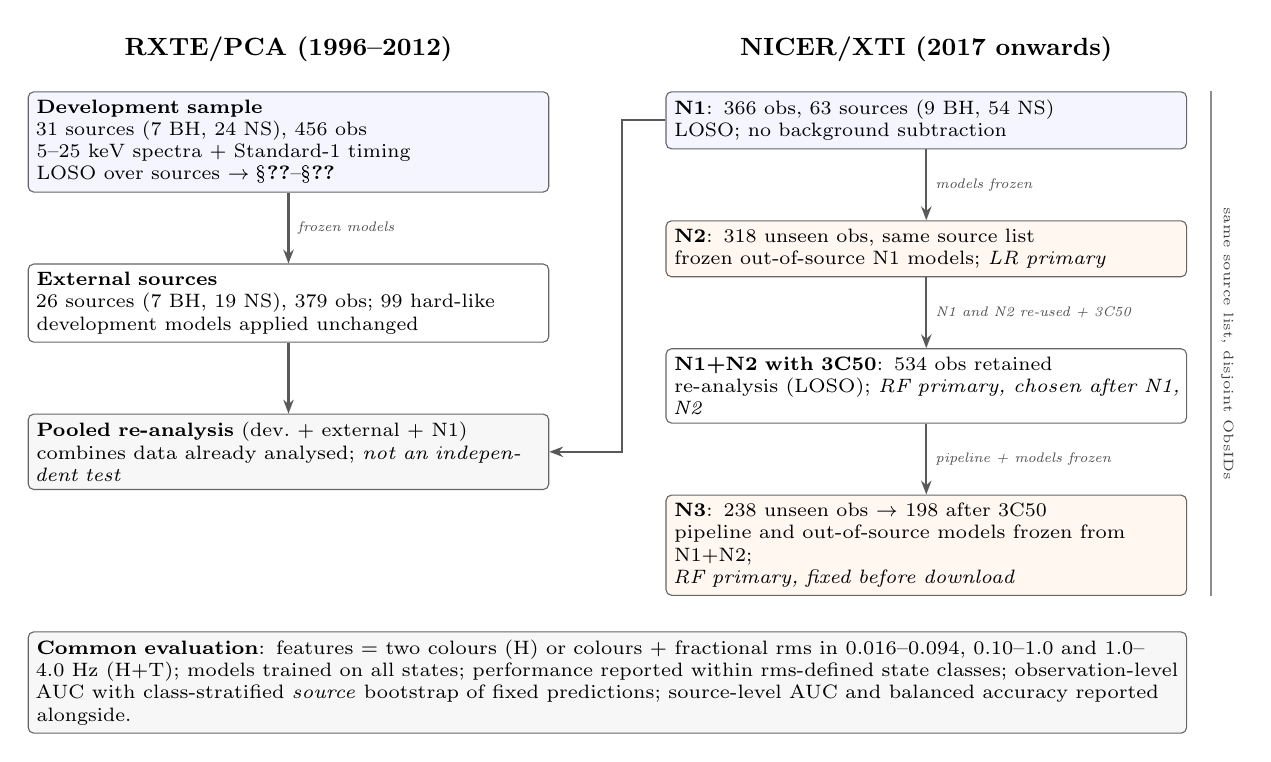
\begin{tikzpicture}[
  font=\scriptsize,
  box/.style={draw=black!60, rounded corners=2pt, align=left, inner sep=3pt, text width=#1, fill=white},
  box/.default=6.4cm,
  hdr/.style={font=\small\bfseries, align=center},
  arr/.style={-{Stealth[length=5pt]}, thick, black!65},
  lab/.style={font=\tiny\itshape, black!70, align=center, fill=white, inner sep=1pt}]
\node[hdr] (hR) at (0,0) {RXTE/PCA (1996--2012)};
\node[hdr] (hN) at (8.1,0) {NICER/XTI (2017 onwards)};
\node[box, below=0.25cm of hR, fill=blue!4] (dev) {\textbf{Development sample}\\31 sources (7 BH, 24 NS), 456 obs\\
  5--25 keV spectra + Standard-1 timing\\LOSO over sources $\rightarrow$ \S\ref{sec:colour}--\S\ref{sec:timing}};
\node[box, below=0.9cm of dev] (ext) {\textbf{External sources}\\26 sources (7 BH, 19 NS), 379 obs; 99 hard-like\\
  development models applied unchanged};
\draw[arr] (dev) -- node[lab, right=2pt] {frozen models} (ext);
\node[box, below=0.25cm of hN, fill=blue!4] (n1) {\textbf{N1}: 366 obs, 63 sources (9 BH, 54 NS)\\LOSO; no background subtraction};
\node[box, below=0.9cm of n1, fill=orange!6] (n2) {\textbf{N2}: 318 unseen obs, same source list\\
  frozen out-of-source N1 models; \emph{LR primary}};
\node[box, below=0.9cm of n2] (n12) {\textbf{N1+N2 with 3C50}: 534 obs retained\\
  re-analysis (LOSO); \emph{RF primary, chosen after N1, N2}};
\node[box, below=0.9cm of n12, fill=orange!6] (n3) {\textbf{N3}: 238 unseen obs $\rightarrow$ 198 after 3C50\\
  pipeline and out-of-source models frozen from N1+N2;\\ \emph{RF primary, fixed before download}};
\draw[arr] (n1) -- node[lab, right=2pt] {models frozen} (n2);
\draw[arr] (n2) -- node[lab, right=2pt] {N1 and N2 re-used + 3C50} (n12);
\draw[arr] (n12) -- node[lab, right=2pt] {pipeline + models frozen} (n3);
\draw[black!45, thick] ($(n1.north east)+(0.3,0)$) -- ($(n3.south east)+(0.3,0)$)
   node[midway, sloped, above, font=\tiny, text=black!75] {same source list, disjoint ObsIDs};
\node[box=6.4cm, below=0.9cm of ext, fill=black!3] (pool) {\textbf{Pooled re-analysis} (dev.\ + external + N1)\\
  combines data already analysed; \emph{not an independent test}};
\draw[arr] (ext) -- (pool);
\draw[arr] (n1.west) -- ++(-0.55,0) |- (pool.east);
\node[box=14.5cm, below=0.45cm of n3.south west, anchor=north west, xshift=-8.1cm, fill=black!3] (ev) {%
  \textbf{Common evaluation}: features = two colours (H) or colours + fractional rms in 0.016--0.094, 0.10--1.0 and
  1.0--4.0~Hz (H+T); models trained on all states; performance reported within rms-defined state classes;
  observation-level AUC with class-stratified \emph{source} bootstrap of fixed predictions; source-level AUC and balanced
  accuracy reported alongside.};
\end{tikzpicture}
\caption{How the samples were used. Arrows show which models or pipelines were carried forward unchanged. Shaded orange
boxes are the two tests on observations that had not been downloaded when the plan for that test was committed. The
pooled re-analysis and the N1+N2 3C50 re-analysis reuse data and are robustness analyses, not independent replications.
All NICER sets draw on one source list, so none of them tests generalisation to new sources.}\label{fig:design}
\end{figure}

% =====================================================================================================
\section{Features, models and evaluation}\label{sec:methods}

\subsection{Colours and spectral representations}\label{sec:colours}
The baseline representation \Hcol{} consists of two hardness ratios of net count rates in detector space. For RXTE they
are $c_1=F(7\text{--}10)/F(5\text{--}7\,\mathrm{keV})$ and $c_2=F(16\text{--}25)/F(10\text{--}16\,\mathrm{keV})$, per
PCU. For NICER they are $c_1=C(4\text{--}6)/C(2\text{--}4\,\mathrm{keV})$ and $c_2=C(6\text{--}10)/C(4\text{--}6\,
\mathrm{keV})$. These are instrument-specific quantities, and no model was transferred between instruments. The RXTE
ablations used five further representations:
\begin{itemize}\setlength\itemsep{1pt}
\item the 45-bin 5--25~keV spectral shape normalised by total flux (B);
\item an intensity-preserving $\mathrm{asinh}$ transform of the spectrum (A);
\item the colours plus log flux (HI);
\item the concatenation \Hcol{}+B;
\item the same quantities on a 3--25~keV grid (H3, B3).
\end{itemize}
For a subset of 396 observations, HEXTE 25--40 and 40--60~keV colours were also available.

\subsection{Low-frequency variability features}\label{sec:timing_features}
Each light curve was divided into 128-s segments. In each segment we computed cross-spectra between independent detector
groups (PCUs for RXTE, MPUs for NICER), averaged over all pairs. Because the Poisson and dead-time noise of different
detectors is uncorrelated, the real part of the cross-spectrum has zero expected white-noise level. Fractional variance
in a band was estimated as the ratio of the summed cross-power to the summed products of mean rates (a ratio of means
over segments). The feature is the signed square root, $T_k=\mathrm{sign}(R_k)\sqrt{|R_k|}$, in three bands:
$T_1$ = 0.016--0.094~Hz, $T_2$ = 0.10--1.0~Hz and $T_3$ = 1.0--4.0~Hz. The bands are the same for both instruments, but
the energy coverage differs: RXTE Standard-1 records all PCA channels without energy resolution, whereas NICER features
use 2--10~keV events. The model with these three features added to the colours is called \HT{}. The models never used
the total rms itself as an input.

\subsection{Operational state classes}\label{sec:states}
Each observation was assigned a state class from its fractional rms $r$, defined as follows:
\begin{itemize}\setlength\itemsep{1pt}
\item $r$ is measured in 0.1--4~Hz for RXTE (limited by Standard-1) and in 0.1--10~Hz for NICER;
\item hard-like: $r>0.10$; soft-like: $r<0.075$; intermediate otherwise;
\item the thresholds are the rms criteria of \citet{RemillardMcClintock2006}, used without their spectral and QPO
criteria.
\end{itemize}
These classes are operational. They are not full spectral-state assignments. Because the RXTE band stops at 4~Hz, its
$r$ is lower than the 0.1--10~Hz value, which makes ``hard-like'' conservative for RXTE. The classes were checked against
expectations: XTE~J1118$+$480 was hard-like in 15 of 15 RXTE observations, and the Z sources Cyg~X-2 and GX~17$+$2 were
soft-like in 27 of 28 RXTE and 15 of 16 NICER observations. Labels were not used to define the classes. All models were
trained on all states, and the classes were used only to stratify the evaluation. The stratifying variable is itself a
variability amplitude that overlaps $T_2$ and $T_3$ in frequency; \cref{sec:unproven} discusses what this implies.

\subsection{Models}\label{sec:models}
We used two classifiers from scikit-learn \citep{Pedregosa2011}:
\begin{itemize}\setlength\itemsep{1pt}
\item a logistic regression (LR) with an $L_2$ penalty ($C=1$), class-balanced weights and standardised inputs;
\item a random forest (RF) with 500 trees, $\sqrt{p}$ features per split, a minimum of two samples per leaf and
class-balanced weights.
\end{itemize}
Hyperparameters were fixed in advance and not tuned. A nested search over eight algorithms is reported only as an
ablation.

\subsection{Evaluation designs and metrics}\label{sec:eval}
Three designs were used.
\begin{enumerate}\setlength\itemsep{1pt}
\item \emph{Leave-one-source-out (LOSO)} within a sample: all observations of a source are scored by a model trained
on all other sources.
\item \emph{Frozen out-of-source prediction} on unseen observations (N2, N3): the observations of source $s$ are scored
by a model trained on the reference data (N1, or the corrected N1+N2) with $s$ removed. Neither the features, the state
thresholds, the background treatment nor the models were changed after the new data were seen.
\item \emph{Frozen external prediction} (RXTE external set): development-sample models applied unchanged.
\end{enumerate}

We distinguish four metrics:
\begin{itemize}\setlength\itemsep{1pt}
\item \emph{observation-level AUC}: the probability that a randomly chosen BH observation receives a higher BH score
than a randomly chosen NS observation, pooling all observations in a stratum, so sources with more observations weigh
more;
\item \emph{observation-level balanced accuracy}: the mean of the BH and NS recalls at the fixed threshold 0.5;
\item \emph{source-level AUC}: computed from source scores, each defined as the mean of the observation scores of that
source;
\item \emph{source-level balanced accuracy}: the same recalls computed on source scores at threshold 0.5.
\end{itemize}
The two source-level metrics weight each source equally. An AUC measures ranking, not accuracy: an AUC of 0.864 does not
mean that 86.4\% of observations are classified correctly.

Intervals are 2.5--97.5 percentiles over 2000 class-stratified bootstrap draws of \emph{sources} (BH and NS sources
resampled separately with replacement, seed 42). In each draw the metric was recomputed on the fixed out-of-sample
predictions; models were not refitted. For stratified metrics, the draws are over all sources of a sample, and the
stratum is applied within each draw. Differences between models are paired within draws. A difference was declared
``detected'' when its interval excluded zero, and ``not detected'' otherwise. These intervals describe source-sampling
variability given fixed predictions. They do not include training variability, measurement error in the features,
label uncertainty, or the multiplicity of analyses across the project.

\subsection{Analysis plans and the status of each result}\label{sec:prereg}
Each analysis round had a plan document committed to the version-controlled repository before the data for that round
were downloaded (\cref{tab:provenance}). We call these \emph{time-stamped, internally pre-specified analysis plans}. Each
plan was written after the results of all earlier rounds were known, and plans were drafted and approved within the
project without external registration or review. Commit timestamps establish the order of events within the repository;
they are not an external registry. Every result below is labelled as one of three types:
\begin{itemize}\setlength\itemsep{1pt}
\item \emph{primary}: the one or two comparisons declared in that round's plan;
\item \emph{descriptive}: other comparisons declared in the plan;
\item \emph{post hoc}: comparisons added after the results were seen.
\end{itemize}
The model class used for the primary hard-like test changed during the project. LR was primary through N2. RF became
primary for the N1+N2 re-analysis after its gains had been seen in earlier rounds. RF was fixed before download only for
N3. No correction for multiple comparisons was applied across rounds.

\begin{table}[t]
\centering\small
\caption{Provenance of the primary hard-like timing tests. ``Plan commit'' is the repository commit that added the plan
document (time UTC+8, 2026). Results are hard-like observation-level AUC differences, \HT{} $-$ \Hcol{}, with 95\%
class-stratified source-bootstrap intervals. All plans were written after the results of earlier rounds.}\label{tab:provenance}
\footnotesize\setlength{\tabcolsep}{4pt}
\footnotesize\setlength{\tabcolsep}{4pt}
\begin{tabular}{@{}p{4.3cm} l l l l@{}}
\toprule
Test (data status) & Plan commit (UTC+8) & Primary model & $\Delta$AUC (95\% interval) & Verdict \\
\midrule
RXTE development (development data) & \texttt{a481fa0}, Oct 5 21:14 & LR & $+0.264$ \ci{+0.048}{+0.455} & detected \\
RXTE external (new sources) & \texttt{a481fa0} & LR, frozen & $+0.064$ \ci{-0.185}{+0.367} & not detected \\
NICER N1 (new instrument) & \texttt{ee4b7db}, Oct 5 23:07 & LR & $+0.112$ \ci{-0.004}{+0.229} & not detected \\
Pooled (re-use of rows 1--3) & \texttt{aeedac7}, Oct 6 00:10 & LR & $+0.145$ \ci{+0.028}{+0.257} & detected$^{a}$ \\
NICER N2 (unseen observations) & \texttt{6fea016}, Oct 6 01:43 & LR, frozen & $+0.066$ \ci{-0.095}{+0.180} & not detected \\
N1+N2 with 3C50 (re-use) & \texttt{2126e9d}, Oct 6 03:13 & RF$^{b}$ & $+0.174$ \ci{+0.071}{+0.300} & detected$^{a}$ \\
NICER N3 (unseen observations) & \texttt{42fe1d2}, Oct 6 04:53 & RF, frozen$^{c}$ & $+0.184$ \ci{+0.049}{+0.337} & detected \\
\bottomrule
\end{tabular}

\smallskip\raggedright\footnotesize
$^{a}$Not an independent test: the data were analysed in earlier rounds. $^{b}$RF chosen as primary after RF gains had
been seen in N1 and N2. $^{c}$RF, the 3C50 pipeline and the out-of-source models were fixed before the N3 data were
downloaded; the N3 data commit is \texttt{6867de0} (05:35) and the results commit \texttt{3d86930} (06:46).
\end{table}

% =====================================================================================================
\section{Results}\label{sec:results}

\subsection{Two colours as a spectral baseline}\label{sec:colour}
On the development sample, LR on the two colours (\Hcol-LR) reached:
\begin{itemize}\setlength\itemsep{1pt}
\item source-level AUC 0.923 \ci{0.804}{0.994};
\item source-level balanced accuracy 0.795 \ci{0.589}{0.958}, with 26 of 31 sources correct (5 of 7 BHs, 21 of 24 NSs);
\item observation-level balanced accuracy 0.776 \ci{0.633}{0.893}.
\end{itemize}
RF on the same colours gave a source-level AUC of 0.905 \ci{0.750}{1.000} (\cref{fig:colour}a). The misclassified
sources under \Hcol-LR were the BHs GRS~1915$+$105 and XTE~J1118$+$480 and the NSs HETE~J1900.1$-$2455, KS~1731$-$260 and
SAX~J1808.4$-$3658.

Adding more spectral information produced no detectable improvement (\cref{fig:colour}b). The source-level AUC
differences relative to \Hcol{} were:
\begin{itemize}\setlength\itemsep{1pt}
\item full 5--25~keV shape (\Hcol+B, primary): $-0.048$ \ci{-0.179}{+0.048} for LR and $-0.012$
\ci{-0.077}{+0.048} for RF;
\item colours including 3--5~keV: $-0.018$ \ci{-0.071}{0.000} for LR and $-0.054$ \ci{-0.161}{+0.006} for RF;
\item 25--60~keV HEXTE colours (396 observations): $-0.048$ \ci{-0.179}{+0.024} for LR and $0.000$
\ci{-0.036}{+0.036} for RF;
\item training \Hcol-LR on all 7949 eligible epoch-5 observations instead of 456: $0.000$ \ci{-0.048}{+0.036};
\item a nested search over eight algorithms and four representations, selected inside the training sources: $-0.173$
\ci{-0.399}{+0.012} relative to \Hcol-LR.
\end{itemize}
Splitting the same data by observation instead of by source inflated observation-level balanced accuracy by $+0.04$ to
$+0.16$, depending on representation and model.

Within the resolution of this sample, the BH/NS information measurable in 5--25~keV PCA spectra is therefore carried by
the two colours. The intervals still allow losses of up to about 0.18 and gains of up to about 0.05 in source-level AUC,
so the results do not establish that the colours contain all of the information, or that the representations are
equivalent.

\begin{figure}[t]
\centering
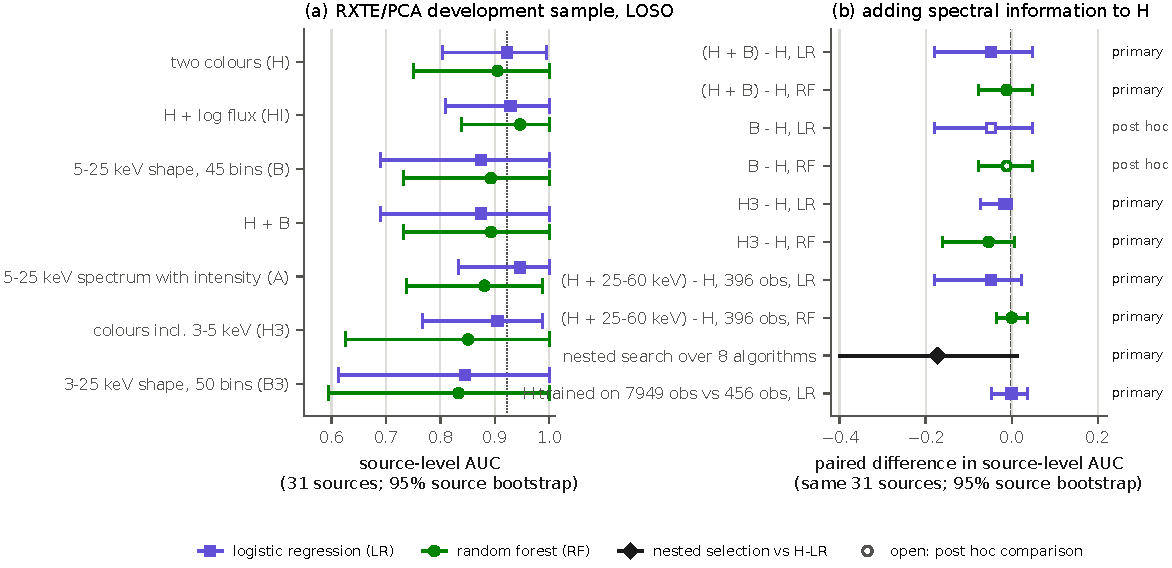
\includegraphics[width=\textwidth]{figures/fig2_colour_ablation.pdf}
\caption{Colour baseline and spectral ablations on the RXTE development sample (31 sources, 456 observations, LOSO).
(a) Source-level AUC (source score = mean observation score) for LR (violet squares) and RF (green circles); the dotted
line marks \Hcol-LR. (b) Paired differences in source-level AUC relative to two colours. ``Primary'' and ``post hoc''
follow the time-stamped plans: the B$-$\Hcol{} comparison was added after the first results. The HEXTE rows use the 396
observations with HEXTE data; the nested search (black diamond) compares an automatically selected model with \Hcol-LR;
the last row compares \Hcol-LR trained on all 7949 eligible epoch-5 observations with \Hcol-LR trained on the 456 used
here, on the same 31 sources. Intervals are 95\% class-stratified source-bootstrap percentiles of fixed LOSO
predictions; they do not include training variability. Source: \texttt{results/v3/v3a\_bootstrap.csv},
\texttt{v3b\_bootstrap.csv}, \texttt{results/v4b3/v4b3\_bootstrap.csv}, \texttt{results/v4/v4a\_bootstrap.csv},
\texttt{results/v4b1/v4b1\_bootstrap.csv}.}\label{fig:colour}
\end{figure}

\subsection{State dependence of colour information}\label{sec:state}
\Cref{fig:states}a--d shows the colour--colour planes split by state class. In soft-like observations, BH and NS
observations occupy largely separate regions in both instruments. In hard-like observations they overlap. In the RXTE
development sample:
\begin{itemize}\setlength\itemsep{1pt}
\item 221 observations were soft-like (38 BH observations from 5 BHs; 183 NS observations from 22 NSs);
\item 180 were hard-like (59 BH observations from all 7 BHs; 121 NS observations from 17 NSs);
\item 55 were intermediate or could not be classified.
\end{itemize}
The \Hcol-LR observation-level AUC was 0.954 \ci{0.801}{1.000} in soft-like observations and 0.646 \ci{0.445}{0.841} in
hard-like ones. The difference, $+0.309$ \ci{+0.099}{+0.510}, was the primary test of that round. RF and the full spectral
shape gave the same pattern, with soft-minus-hard differences of $+0.254$ for \Hcol-RF and $+0.293$ for B-LR, both with
intervals excluding zero.

The same ordering holds in every NICER set (\cref{fig:states}e). Colour-only hard-like AUCs were 0.50--0.68 for LR and
0.67--0.75 for RF, against soft-like AUCs of 0.83--0.95. These NICER values are descriptive. Two features of the design
matter for interpretation. Only five BHs contribute soft-like RXTE observations, so the soft-like AUC is uncertain. And
the hard-like class contains all seven RXTE BHs, so the hard-like problem is the one that every BH source poses at some
time.

\begin{figure}[t]
\centering
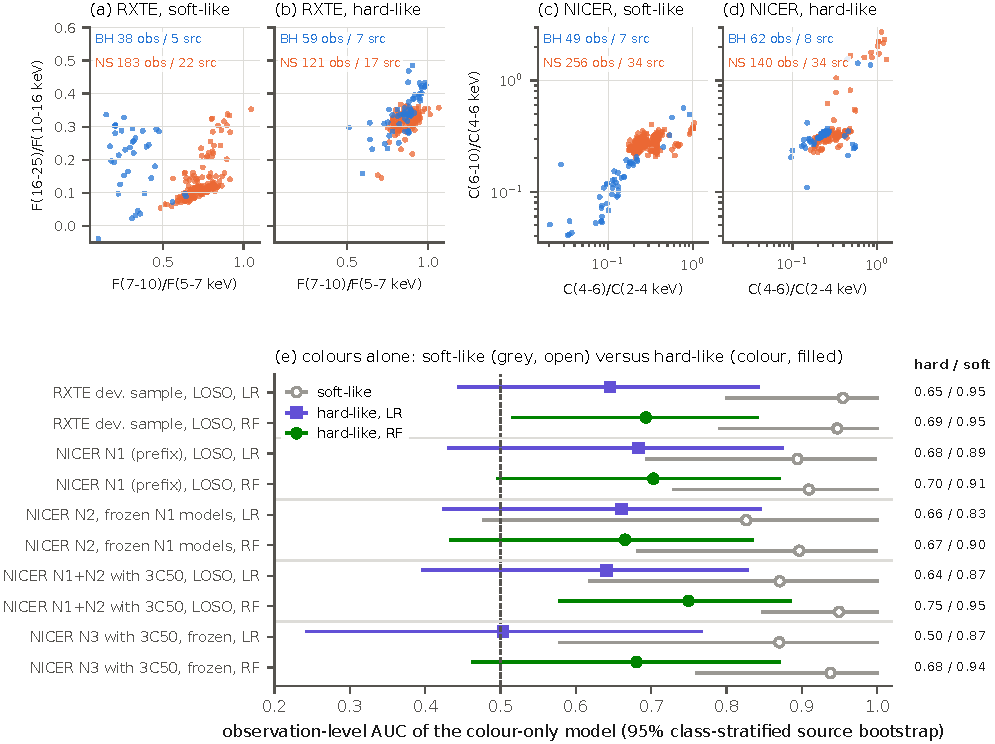
\includegraphics[width=\textwidth]{figures/fig3_states.pdf}
\caption{State dependence of the colour information. (a--d) Colour--colour planes for soft-like ($r<0.075$) and
hard-like ($r>0.10$) observations, where $r$ is the fractional rms in 0.1--4~Hz (RXTE) or 0.1--10~Hz (NICER). RXTE:
development sample; NICER: N1+N2 after 3C50 correction and screening. Colours are detector-space count ratios and are not
comparable between instruments; NICER axes are logarithmic. Intermediate observations are not shown. (e) Observation-level
AUC of colour-only models in soft-like (grey, open) and hard-like (colour, filled) observations. Only the RXTE \Hcol-LR
soft-minus-hard difference was a primary test; the NICER rows are descriptive. Intervals are 95\% class-stratified source
bootstrap of fixed out-of-sample predictions; numbers at right are the point estimates. Source:
\texttt{results/v7a/states.csv}, \texttt{state\_stratified\_metrics.csv}, \texttt{results/v9a/v9a\_metrics.csv},
\texttt{results/v11/v11a\_metrics.csv}, \texttt{results/v12/v12b\_gain.csv}, \texttt{results/v13/v13a\_gain.csv},
\texttt{data/v12/processed/nicer\_corrected\_screened.csv}.}\label{fig:states}
\end{figure}

\subsection{Low-frequency variability within hard-like observations}\label{sec:timing}
\Cref{fig:gain} collects every hard-like comparison of \HT{} with \Hcol{} using the same model class. Rows are grouped by
sample and annotated with data status, background treatment, role, and when the model was fixed.

\paragraph{RXTE.}
In the development sample, adding $T_1$--$T_3$ raised the \HT-LR hard-like observation-level AUC from 0.646 to 0.910, a
gain of $+0.264$ \ci{+0.048}{+0.455} (primary). The other comparisons in this sample were descriptive:
\begin{itemize}\setlength\itemsep{1pt}
\item with RF the gain was $+0.230$ \ci{+0.074}{+0.408};
\item in soft-like observations, where the colours already separate the classes, the LR gain was $+0.036$
\ci{0.000}{+0.158};
\item at source level within hard-like observations, the AUC rose from 0.748 to 0.933 ($+0.185$ \ci{+0.008}{+0.403}).
\end{itemize}
On the external RXTE sources, frozen development-sample models gave a hard-like gain of $+0.064$ \ci{-0.185}{+0.367}
(primary, not detected; 99 observations of 5~BHs and 15~NSs). The colour-only baseline on these sources was already 0.817.
Some sources moved in the right direction: GS~1354$-$64 rose from a mean BH score of 0.54 to 0.97. Others moved the wrong
way: the NSs IGR~J00291$+$5934 and EXO~1745$-$248 rose from 0.45 to 0.89 and from 0.32 to 0.73 respectively.

\paragraph{NICER N1.}
With LR the gain was $+0.112$ \ci{-0.004}{+0.229} (primary, not detected). With RF it was $+0.236$ \ci{+0.104}{+0.372}
(descriptive). Using the full event files gave $+0.107$ \ci{-0.010}{+0.224} with LR and $+0.219$ \ci{+0.100}{+0.337} with
RF. Adding the bands one at a time to the colours with LR gave $+0.048$ \ci{-0.041}{+0.140} for $T_1$, $+0.143$
\ci{+0.028}{+0.271} for $T_2$ and $+0.115$ \ci{+0.030}{+0.217} for $T_3$. In RXTE, by contrast, $T_1$ alone gave the
largest single-band improvement (hard-like AUC 0.926, against 0.874 for $T_2$ and 0.654 for $T_3$). Which frequency band
carries the information is therefore not stable across instruments, whose energy coverage also differs. Controlling for
brightness with the log count rate as an extra input reduced the N1 LR gain to $+0.069$ \ci{-0.013}{+0.161}. The pooled
RXTE+NICER test gave $+0.145$ \ci{+0.028}{+0.257}, but it combines data already analysed and is not independent of the
rows above it.

\paragraph{Summary.}
Before any test on unseen observations, every point estimate of the hard-like timing gain was positive. With LR, only the
RXTE development interval excluded zero. With RF, every interval excluded zero, but RF was not yet a primary model.

\begin{figure}[t]
\centering
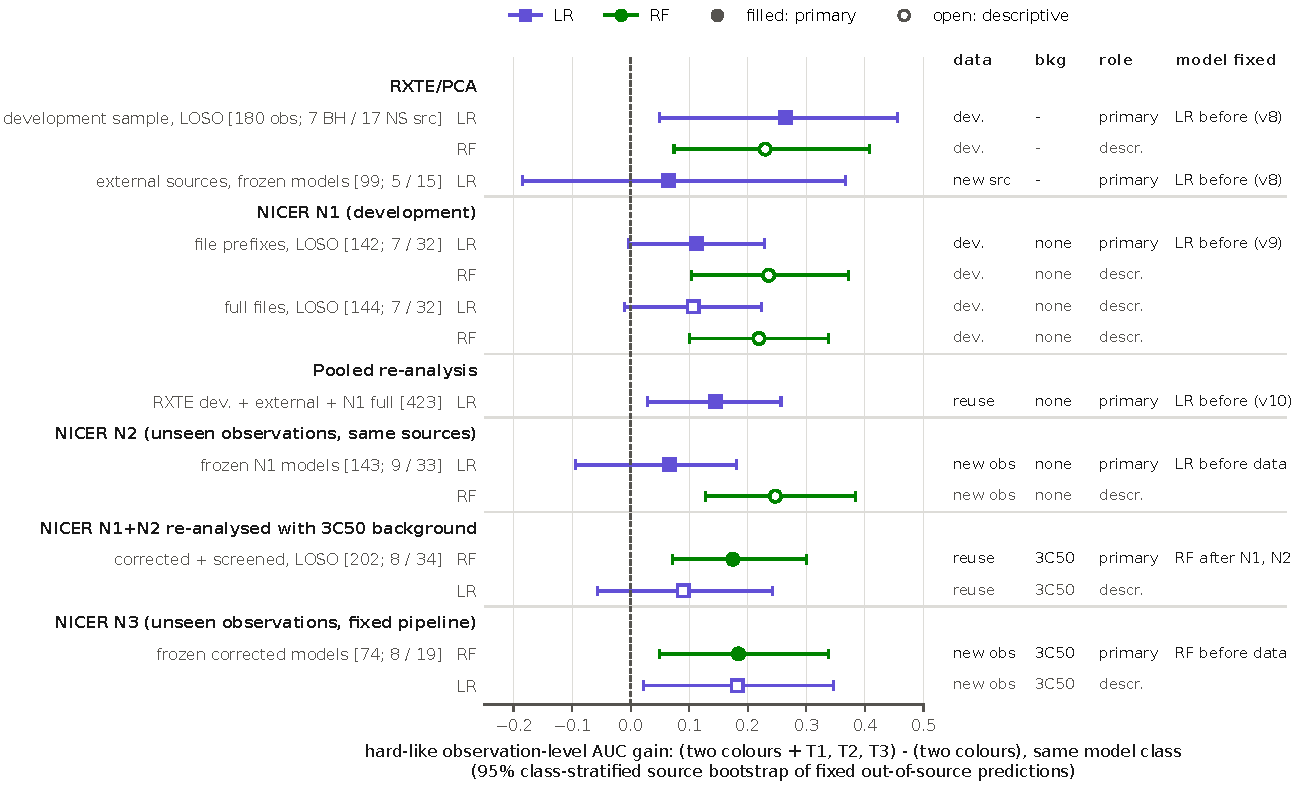
\includegraphics[width=\textwidth]{figures/fig4_timing_gain.pdf}
\caption{Hard-like observation-level AUC gain from adding fractional rms in 0.016--0.094, 0.10--1.0 and 1.0--4.0~Hz to
two colours, for the same model class (LR violet squares; RF green circles). Filled: primary comparison of that round's
plan; open: descriptive. Brackets give hard-like observations and BH/NS sources. ``Data'' marks development data used to
form the hypothesis (dev.), sources never used in training (new src), observations never analysed before (new obs), or
re-analysis of data already analysed (reuse). ``Model fixed'' gives when the primary model class was fixed relative to
the data; all plans were written after earlier results. Rows sharing data are not independent: the pooled row combines
the RXTE and N1 rows, and the 3C50 row re-analyses N1 and N2. Intervals: 95\% class-stratified source bootstrap of fixed
predictions, excluding training variability. Source: \texttt{results/final\_timing\_gain\_across\_versions.csv};
\texttt{results/v10a/v10a\_pooled\_gain.csv} for the N1 full-file LR row.}\label{fig:gain}
\end{figure}

\subsection{Background robustness and tests on unseen observations}\label{sec:robust}
\paragraph{N2: unseen observations, LR fixed in advance.}
The primary LR gain on 143 hard-like N2 observations was $+0.066$ \ci{-0.095}{+0.180}, which was not detected. The LR
colour-only AUC was 0.660 and \HT-LR reached 0.726. At the frozen 0.5 threshold, \HT-LR had a \emph{lower}
observation-level balanced accuracy than \Hcol-LR ($-0.080$ \ci{-0.166}{-0.022}), indicating that its calibration did not
carry over to the new observations. The RF gain on the same observations was $+0.247$ \ci{+0.128}{+0.384} (0.665 to 0.912;
descriptive).

\paragraph{N1+N2 with 3C50 background correction.}
After correction and screening, the RF gain was $+0.174$ \ci{+0.071}{+0.300} (0.750 to 0.924; 202 hard-like observations
of 8~BHs and 34~NSs). RF was made primary for this round after its gains had been seen in N1 and N2, and the data are
re-used, so this result tests robustness to the background treatment. It is not an independent confirmation. The LR gain
was $+0.090$ \ci{-0.056}{+0.243}. At source level, the RF AUC gain was $+0.074$ \ci{-0.033}{+0.206} and the balanced-accuracy
gain $+0.173$ \ci{+0.004}{+0.357}. The background correction itself changed little: the median background fraction was
below one per cent.

\paragraph{N3: unseen observations, fixed pipeline, RF fixed in advance.}
The background treatment, state thresholds, features and out-of-source RF models were all frozen before the N3 data were
downloaded. The 74 hard-like N3 observations comprise 29 observations of 8~BHs and 45 of 19~NSs. Their composition is
uneven: Cyg~X-1 contributes 7 of the BH observations and 4U~1812$-$12 contributes 8 of the NS observations. The
observation-level AUC rose from 0.680 \ci{0.463}{0.870} for \Hcol-RF to 0.864 \ci{0.714}{0.968} for \HT-RF, a gain of
$+0.184$ \ci{+0.049}{+0.337} (primary, detected; \cref{tab:v13}, \cref{fig:v13}). The descriptive checks were:
\begin{itemize}\setlength\itemsep{1pt}
\item LR showed a similar gain, $+0.182$ \ci{+0.022}{+0.347}, from a colour-only AUC of 0.503;
\item the soft-like RF gain was $+0.005$ \ci{-0.015}{+0.035};
\item observation-level balanced accuracy at the frozen threshold rose by $+0.137$ \ci{+0.019}{+0.275};
\item removing one BH source at a time left gains between $+0.146$ and $+0.212$;
\item recomputing the timing features of 106 faint observations within the 3C50 GTIs gave $+0.190$ \ci{+0.065}{+0.330}.
\end{itemize}
At source level (27 sources with hard-like observations), the AUC rose from 0.717 to 0.842, a gain of $+0.125$
\ci{-0.053}{+0.303}, and the balanced-accuracy gain was $+0.099$ \ci{-0.053}{+0.286}. Neither was detected. The
pre-specified test therefore confirms an observation-level gain on unseen observations. With equal weight per source the
gain points in the same direction, but this sample cannot resolve it.

\begin{table}[t]
\centering\small
\caption{NICER N3 (unseen observations; frozen 3C50 pipeline; out-of-source models trained on corrected N1+N2).
Point estimates with 95\% class-stratified source-bootstrap intervals of fixed predictions. Observation-level rows use
all sources of N3 in each draw; source-level rows and the observation balanced accuracy use a paired bootstrap over the
27 sources with hard-like observations.}\label{tab:v13}
\footnotesize\setlength{\tabcolsep}{2.7pt}
\begin{tabular}{@{}l l l l l@{}}
\toprule
Metric (hard-like unless stated) & Colours only & + $T_1$--$T_3$ & Difference & Role \\
\midrule
Observation AUC, RF (74 obs) & 0.680 \ci{0.463}{0.870} & 0.864 \ci{0.714}{0.968} & $+0.184$ \ci{+0.049}{+0.337} & primary \\
Observation AUC, LR & 0.503 \ci{0.242}{0.766} & 0.685 \ci{0.375}{0.940} & $+0.182$ \ci{+0.022}{+0.347} & descr. \\
Obs.\ balanced accuracy, RF & 0.607 \ci{0.430}{0.769} & 0.744 \ci{0.557}{0.897} & $+0.137$ \ci{+0.019}{+0.275} & descr. \\
Source AUC, RF (27 src) & 0.717 \ci{0.507}{0.895} & 0.842 \ci{0.671}{0.961} & $+0.125$ \ci{-0.053}{+0.303} & descr. \\
Source balanced accuracy, RF & 0.572 \ci{0.421}{0.750} & 0.671 \ci{0.467}{0.859} & $+0.099$ \ci{-0.053}{+0.286} & descr. \\
Soft-like observation AUC, RF & 0.938 \ci{0.760}{1.000} & 0.943 \ci{0.772}{1.000} & $+0.005$ \ci{-0.015}{+0.035} & descr. \\
Obs.\ AUC, RF, 3C50-GTI timing & --- & --- & $+0.190$ \ci{+0.065}{+0.330} & descr. \\
Obs.\ AUC, RF, leave one BH out & --- & --- & $+0.146$ to $+0.212$ (8 values) & influence \\
\bottomrule
\end{tabular}
\end{table}

\begin{figure}[t]
\centering
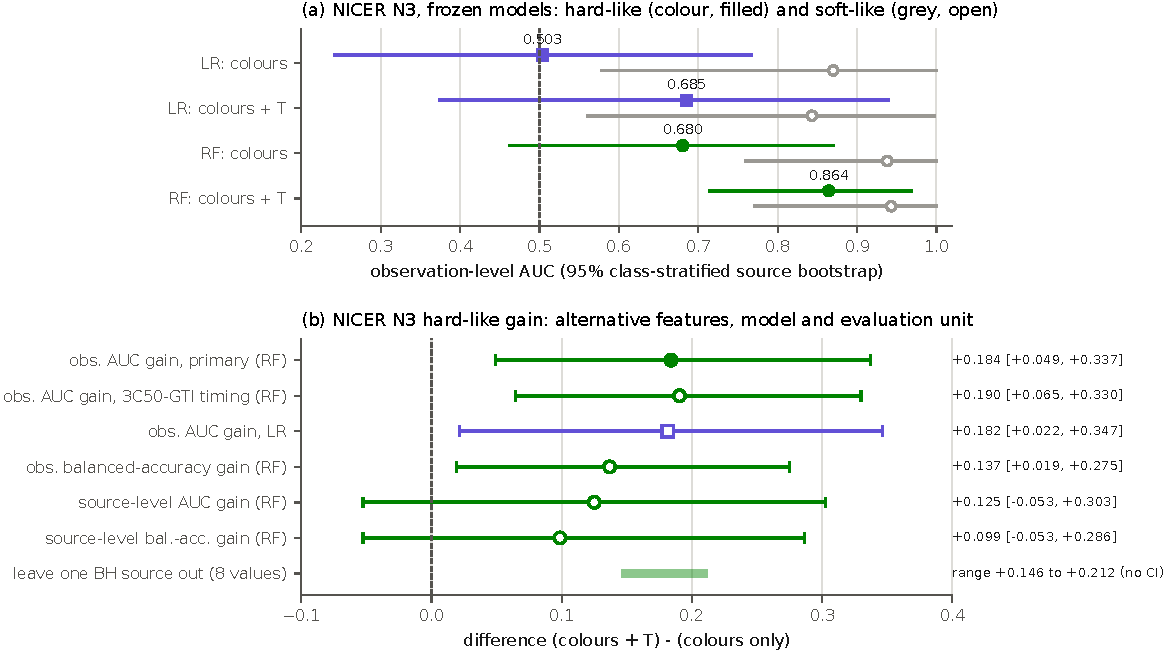
\includegraphics[width=0.95\textwidth]{figures/fig5_v13.pdf}
\caption{The N3 test on unseen NICER observations. (a) Observation-level AUC of frozen out-of-source models in hard-like
(colour, filled; 74 observations, 8 BH/19 NS sources) and soft-like (grey, open; 120 observations) observations; numbers
are hard-like point estimates. (b) Hard-like gain from adding $T_1$--$T_3$, under the primary specification (filled) and
descriptive alternatives: timing features recomputed within the 3C50 good-time intervals for 106 faint observations; LR
instead of RF; observation-level balanced accuracy at the frozen 0.5 threshold; source-level AUC and balanced accuracy
(each source weighted equally); and the range of the primary gain when one BH source is removed at a time (bar; no
interval). Note that rows use different metrics. Intervals: 95\% class-stratified source bootstrap of fixed predictions.
Source: \texttt{results/v13/v13a\_gain.csv}, \texttt{v13a\_gti\_restricted.csv}, \texttt{v13a\_influence.csv}.}\label{fig:v13}
\end{figure}

\subsection{Secondary result: characteristic frequency at matched colour}\label{sec:nuc}
We also asked whether, at matched colours, BHs have a lower characteristic variability frequency $\nuc$. Here $\nuc$ is
the power-weighted geometric-mean frequency of the 0.008--64~Hz (NICER) or 0.008--4~Hz (RXTE) cross-spectrum. The test
proceeds in three steps:
\begin{enumerate}\setlength\itemsep{1pt}
\item residualise $\log_{10}\nuc$ on the colours with a label-blind $k$-nearest-neighbour regression;
\item average the residuals within each source;
\item compare the BH and NS means by permuting source labels.
\end{enumerate}
The details are in \cref{app:nuc}. The BH-minus-NS difference $D$ was negative in every NICER set and in RXTE hard-like
data ($-0.27$ to $-0.66$~dex), but its significance varied:
\begin{itemize}\setlength\itemsep{1pt}
\item the pooled test gave $p=0.0012$, but it re-uses data;
\item in N2, $D=-0.66$ ($p=0.022$) weakened to $-0.46$ ($p=0.19$) when very hard observations, likely dominated by
background, were removed post hoc;
\item after 3C50 correction, N1+N2 gave $D=-0.51$ ($p=0.073$);
\item N3 gave $D=-0.43$ ($p=0.21$) under the primary pipeline and $D=-0.30$ ($p=0.41$) with timing restricted to the
3C50 GTIs;
\item the RXTE external sources showed no difference ($D=-0.04$, $p=0.78$).
\end{itemize}
We regard this as a consistent but unconfirmed lead. It is not evidence for mass scaling, because neither Eddington ratio
nor mass was controlled.

% =====================================================================================================
\section{Discussion}\label{sec:discussion}

\subsection{What has been learned beyond classification accuracy}\label{sec:learned}
\emph{Where the spectral signal lives.} In the RXTE development sample, two hardness ratios reproduce the source-level
performance of full-spectrum representations. Neither more bands, more observations nor more flexible models added
detectable information. This connects the classification problem to the colour--colour phenomenology of
\citet{DoneGierlinski2003}. It also suggests, without testing it, that spectral classifiers trained on similar PCA data
\citep{Pattnaik2021} may rely largely on the same two-colour information. We did not evaluate those models, so this
remains a hypothesis.

\emph{Where it fails.} The colour information is concentrated in soft-like observations. In hard-like observations,
colour-only AUCs of 0.50--0.75 across five samples show that BH and NS colours overlap substantially. This quantifies,
with intervals that respect source clustering, the state dependence noted by \citet{Pattnaik2021}. It is also consistent
with \citet{Burke2017}, whose hard-state differences lie in Comptonization parameters that 2--25~keV count colours sample
only weakly.

\emph{What variability adds.} Within hard-like observations, adding three low-frequency rms amplitudes to the colours
increased the observation-level AUC (point estimate) in every sample analysed. As a primary test, the increase was
detected in the RXTE development sample, in the N1+N2 3C50 re-analysis, and in the N3 test with a pipeline and model
fixed before download; it was not detected in the RXTE external set, in N1 with LR, or in N2 with LR. The gain was absent in soft-like observations, where colours already separate the classes, so
timing complements colours rather than replacing them. This is not the high-frequency criterion of
\citet{SunyaevRevnivtsev2000}. Our exploratory event-mode analysis found 512--1024~Hz power detectable in only 1 of 17 NSs
in single RXTE observations, and its implementation check failed (\cref{app:extra}). Nor does the result contradict the
broad similarity of BH and NS power colours \citep{Heil2015,GardenierUttley2018}: tracks that are similar overall can
still differ in amplitude at a given colour.

\emph{How robust the gain is to modelling choices.} RF gains were consistently $+0.17$ to $+0.25$. LR gains ranged from
$+0.07$ to $+0.26$, and LR calibration failed to transfer to N2. This points to a non-linear or threshold-like relation
between colours, rms and class, but it is not a mechanism. The band that matters also differed between instruments ($T_1$
for RXTE, $T_2$ and $T_3$ for NICER), and the two instruments sample different energies. We therefore do not attribute the
gain to a particular power-spectral component.

\subsection{What remains unproven}\label{sec:unproven}
\begin{enumerate}\setlength\itemsep{2pt}
\item \emph{Generalisation to new sources.} N2 and N3 are new observations of sources already in the sample. The
out-of-source models never trained on the tested source, but the source population, and the hypotheses, came from the
same sources. Observations of one outburst are correlated. In N3 the source-level gain ($+0.125$) was not detected.
Confirmation needs BHs not yet used, such as future transients.
\item \emph{One confirmatory test of the RF specification.} RF became the primary model only after its gains had been
seen. N3 is the only test in which it was fixed before download. The N1+N2 re-analysis and the pooled test re-use data
and are not replications.
\item \emph{Selection on a timing quantity.} Hard-like observations are selected by $r>0.10$, a variability amplitude
that overlaps $T_2$ and $T_3$. Labels were not used, and both models are evaluated on the same subset, so this selection
does not by itself create a spurious gain. It does mean that the result is conditional on an rms-defined subset, not on a
spectrally defined hard state, and that a practical classifier needs timing to identify the stratum. A natural question
is whether a single total rms adds as much as the three bands. We did not compare colours plus total rms with colours
plus $T_1$--$T_3$, so we cannot say whether band structure or amplitude alone carries the information.
\item \emph{Weighting and dependence.} Observation-level AUCs weight sources by their number of observations. Source-level
metrics give equal weight but have little power with 8 BHs. We did not run a source-equal-weight observation-level
analysis, nor one blocked by outburst.
\item \emph{Background and selection effects.} The 3C50 failures (mainly early gain-calibration files) are not random.
Background time variability is not modelled. The mismatch between 3C50 and timing GTIs was checked only for N3.
\item \emph{Physical confounders.} Eddington ratio, inclination and NS subclass (atoll, Z source, accreting millisecond
pulsar) were not controlled; only a count-rate proxy for brightness was tried.
\item \emph{Uncertainty.} The bootstrap intervals include source sampling only. They exclude refitting variability,
measurement error in the features and the labels, and the multiplicity of comparisons made over the project.
\end{enumerate}

\subsection{How this extends prior work}\label{sec:prior}
Several elements are not new: evaluation with sources held out \citep{Pattnaik2021,deBeurs2022}, the observation that hard
and intermediate states are harder to classify \citep{Pattnaik2021}, and the use of timing to separate BHs from NSs
\citep{SunyaevRevnivtsev2000,WijnandsvanderKlis1999,KleinWolt2008}. What this work adds is narrower:
\begin{itemize}\setlength\itemsep{1pt}
\item an ablation showing that two colours carry the detectable PCA spectral information in this sample;
\item an estimate of the state dependence with source-level uncertainty;
\item a specific test of whether low-frequency variability adds information beyond colours within hard-like
observations of held-out sources, repeated across two instruments and a background re-analysis, and confirmed once on
unseen observations with a frozen pipeline.
\end{itemize}

The observation-split evaluation of \citet{Garg2026} answers a different question, namely recognition of sources already
seen in training. In our data, splitting by observation inflated balanced accuracy by 0.04--0.16, but we did not evaluate
their model, and we do not claim that it fails on new sources. Their ``variance of the data'' is a spectral statistic,
not a Fourier timing feature, so the two results are not directly comparable. For MAXI colours (\cref{app:extra}), we
reproduced the published results of \citet{deBeurs2022}. With strictly dynamical BH labels, linear models on MAXI colours
had little discriminating power, while non-linear models reached a source-level AUC near 0.8. The samples, labels and
metrics differ, so these numbers do not rank the methods. No result here supports claims of being first, of state-of-the-art
performance, or of outperforming earlier work.

\subsection{Next steps}\label{sec:next}
The most informative next step is to apply the frozen N3 pipeline and RF model, without changes, to BH and NS sources
never used here, for example new transients observed by NICER. Before that, analyses that could change the interpretation
can be done with existing data:
\begin{itemize}\setlength\itemsep{1pt}
\item colours plus total rms against colours plus $T_1$--$T_3$;
\item source-equal-weight and outburst-blocked versions of the hard-like gain;
\item matching the 3C50 and timing GTIs in all NICER sets;
\item a fair comparison with published models on identical data and splits.
\end{itemize}
These are listed, with priorities, in the accompanying document for discussion.

% =====================================================================================================
\section{Conclusions}\label{sec:conclusions}
\begin{enumerate}\setlength\itemsep{2pt}
\item For RXTE/PCA 5--25~keV spectra of 31 held-out sources, two hardness ratios gave a source-level AUC of 0.923
\ci{0.804}{0.994}. No other spectral representation, energy band, sample size or model search tried here added detectable
information. This is not evidence that the colours contain all of the information.
\item Colour information is state dependent. The observation-level AUC was 0.954 for soft-like and 0.646 for hard-like
RXTE observations (difference $+0.309$ \ci{+0.099}{+0.510}). Every NICER set showed the same ordering.
\item Within rms-defined hard-like observations, adding 0.016--4~Hz rms amplitudes to the colours increased the
observation-level AUC in every sample. On 198 unseen NICER observations with a frozen pipeline and a random forest fixed
before download, the hard-like AUC rose from 0.680 to 0.864 ($+0.184$ \ci{+0.049}{+0.337}). The source-level gain
($+0.125$ \ci{-0.053}{+0.303}) was not detected.
\item All tests on new data used the same sources. Confirmation on new BHs is the decisive missing step.
\item A lower characteristic variability frequency of BHs at matched colour is a consistent but unconfirmed secondary
lead. It does not support any claim about mass scaling, event horizons or new physics.
\end{enumerate}

% =====================================================================================================
\section*{Acknowledgements}
\placeholder{Acknowledgements, funding and computing resources to be supplied by the authors.} This research used data
and software provided by the High Energy Astrophysics Science Archive Research Center (HEASARC) at NASA/GSFC, data from
the RXTE and NICER missions, and the MINBAR burst catalogue. \placeholder{Decide whether and how to disclose AI
assistance in analysis and writing, according to the target journal's policy.}

\section*{Data and code availability}
All analysis code, configuration files, time-stamped analysis plans, decision logs and result tables are in the
repository \url{https://github.com/Chipwwwwww/XRB-pilot} \placeholder{confirm public visibility and archive with a DOI}.
This draft uses commit \texttt{666c2e0}. Raw RXTE and NICER data are public at HEASARC. Download URLs, byte counts and
SHA-256 checksums are logged in \texttt{logs/downloads.jsonl}. Figures~2--5 and C.1 were redrawn from committed result
files by \texttt{paper\_draft/scripts/make\_figures.py}, without re-running any analysis.

\bibliographystyle{plainnat}
\bibliography{references}

% =====================================================================================================
\appendix
\counterwithin{figure}{section}
\counterwithin{table}{section}
\section{Correspondence with the repository analysis rounds}\label{app:versions}
The repository records the work as numbered rounds (v1--v14), each with its own plan, script set and result directory.
\Cref{tab:versions} maps them to the sections of this paper. The rounds are listed for traceability only; the paper is
organised by scientific question.

\begin{table}[h]
\centering\footnotesize
\caption{Repository rounds used in this paper. ``Plan'' files are \texttt{reports/preregistration\_vN.md}; results are under
\texttt{results/vN*/}.}\label{tab:versions}
\begin{tabularx}{\textwidth}{@{}l X l@{}}
\toprule
Round & Content used here & Section \\
\midrule
v1--v2 & RXTE pilot (8 sources) and development sample (31 sources), LOSO, representations A, B, H, HI & \ref{sec:rxte}, \ref{sec:colour} \\
v3 & nested increment \Hcol+B$-$\Hcol, 3--25~keV band, BH candidates (descriptive) & \ref{sec:colour}, \ref{app:extra} \\
v4 & algorithm search, burst check, HEXTE, earlier gain epochs, all observations & \ref{sec:colour}, \ref{app:extra} \\
v5--v6 & Standard-1 timing features, external sources, permutation test & \ref{sec:timing_features}, \ref{app:nuc} \\
v7 & state classes, MINBAR burst exclusion, persistent BHs, MAXI & \ref{sec:states}, \ref{sec:state}, \ref{app:extra} \\
v8 & hard-like timing gain (RXTE), external hard-like test, event-mode high frequencies, MAXI $N_{\rm H}$ & \ref{sec:timing}, \ref{app:extra} \\
v9--v10 & NICER N1, pooled RXTE+NICER & \ref{sec:nicer}, \ref{sec:timing} \\
v11 & NICER N2 (unseen observations, frozen models) & \ref{sec:robust} \\
v12 & 3C50 background re-analysis of N1+N2 & \ref{sec:bkg}, \ref{sec:robust} \\
v13 & NICER N3 (unseen observations, frozen pipeline, RF fixed) & \ref{sec:robust} \\
v14 & cross-round summary (no new analysis) & --- \\
\bottomrule
\end{tabularx}
\end{table}

\section{Additional results}\label{app:extra}
The following results support the main text but are not part of its argument. All are taken from committed result files.
\begin{itemize}\setlength\itemsep{2pt}
\item \emph{Burst contamination (v4, v7).} Matching the 456 development observations to MINBAR within the PCA field of
view flagged 58 observations, all NSs. Excluding them did not change the colour-baseline or full-spectrum conclusions.
\item \emph{BH candidates (v3c).} Fourteen BlackCAT candidates were scored with models trained on confirmed sources. This
is descriptive only, and the candidates were never used as labels.
\item \emph{External sources, all states (v6).} Frozen colour models reached a source-level AUC of 1.000 with and
without timing on 23 external sources. Source-level balanced accuracy rose from 0.868 to 0.974 ($+0.105$
\ci{0.000}{+0.237}), which was not detected.
\item \emph{MAXI (v7, v8, v9).} The published MAXI results of \citet{deBeurs2022} were reproduced from their public
data. With dynamically confirmed BHs only (13 BHs and 48 non-pulsing NSs), LR on MAXI colours gave source-level AUCs of
0.56--0.59. Neither primary comparison was detected. $k$-nearest-neighbour models on two colours reached 0.80. Adding a
colour that includes the 2--4~keV band to a single $\geq4$~keV colour still helped after correcting for Galactic
$N_{\rm H}$ (RF $+0.377$ \ci{+0.160}{+0.595}). However, the corrected single-colour comparison model had a source-level AUC of only
0.361, so part of this gain reflects a baseline below chance.
\item \emph{High-frequency timing (v8).} RXTE event-mode cross-spectra (4--1024~Hz) failed a pre-specified
implementation check (Spearman correlation 0.81--0.82 with Standard-1 features, against the required 0.90), so all results are
exploratory. After a post hoc subtraction of a white component common to the PCUs, 512--1024~Hz power was detected
above $3\sigma$ in 1 of 17 NSs and in none of 6 BHs. High-frequency features added little beyond the low-frequency ones
(RF $+0.009$).
\end{itemize}

\section{Characteristic frequency: definition and full results}\label{app:nuc}
For NICER, $\nuc=\exp\!\left(\sum_b w_b\ln\nu_b/\sum_b w_b\right)$ over 13 octave bins between 1/128 and 64~Hz, with
$w_b=\max(P_b,0)$ the band cross-power. $\nuc$ is missing when the total rms in these bins is below 0.05. The RXTE
definition (9 bins, 1/128--4~Hz) divides $w_b$ by the logarithmic bin width; the two definitions are therefore not
identical. The test proceeds as follows:
\begin{enumerate}\setlength\itemsep{1pt}
\item residualise $\log_{10}\nuc$ on standardised colours with a $k=25$ nearest-neighbour regression that excludes the
observation's own source and ignores labels;
\item average the residuals per source;
\item take $D$ = mean(BH) $-$ mean(NS);
\item permute source labels 20\,000 times; the $p$-value is two-sided.
\end{enumerate}
\Cref{fig:nuc} lists all primary, descriptive and post hoc results. Frozen thresholds $\nu^{*}$ were also defined before
N2 and N3 (1.30 and 1.336~Hz; a hard-like observation with $\nuc<\nu^{*}$ is classified as a BH). In N3 this rule gave
observation-level sensitivity 0.79 and specificity 0.76, and at source level classified 7 of 8 BHs and 13 of 19 NSs
correctly.

\begin{figure}[h]
\centering
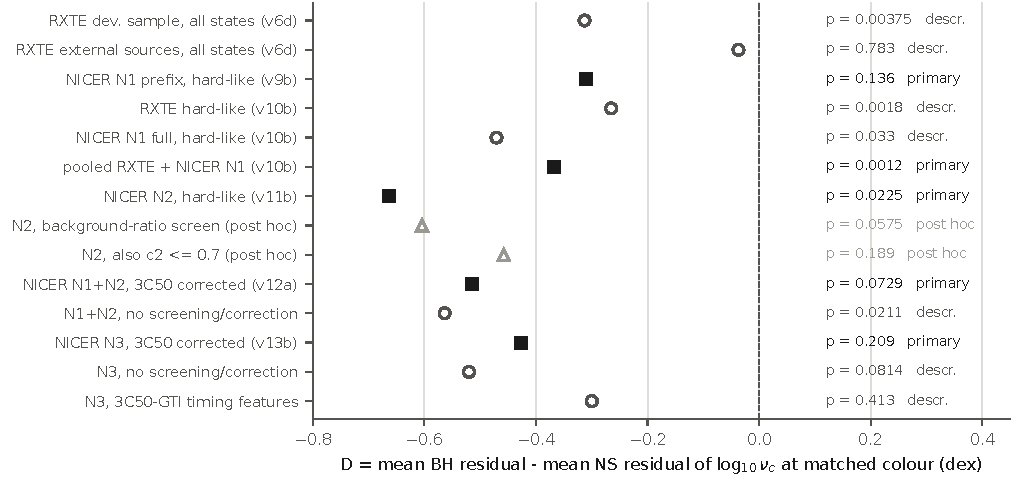
\includegraphics[width=0.95\textwidth]{figures/figA1_nuc.pdf}
\caption{Colour-conditional difference in $\log_{10}\nuc$ between BH and NS sources (negative: BHs lower at matched
colour). Squares: primary tests; circles: descriptive; triangles: post hoc. $p$-values from 20\,000 source-label
permutations. Rows share data (the pooled and 3C50 rows re-use earlier sets), so the $p$-values are not independent, and
no multiplicity correction is applied. Source: \texttt{results/final\_nuc\_difference\_across\_versions.csv},
\texttt{results/v11/v11b\_post\_hoc\_screens.csv}, \texttt{results/v12/v12a\_nuc.csv},
\texttt{results/v13/v13b\_nuc.csv}.}\label{fig:nuc}
\end{figure}

\section{Literature comparison}\label{app:lit}
\Cref{tab:lit} contrasts the designs; it is not a ranking of performance. The bibliographic fields were verified
against search-engine records of arXiv, ADS and publisher pages on 2026 October 9. The full texts could not be retrieved
from the writing environment, so method details for \citet{Garg2026} (observation-wise 80:20 split) and the state remark
in \citet{Pattnaik2021} come from the project's earlier reading of those papers and should be re-checked
(\placeholder{verify against full text}).

\begin{table}[h]
\centering\footnotesize
\caption{Design comparison with related machine-learning work. Numbers are not comparable across rows.}\label{tab:lit}
\begin{tabularx}{\textwidth}{@{}l *{4}{>{\raggedright\arraybackslash}X}@{}}
\toprule
 & \citet{Pattnaik2021} & \citet{deBeurs2022} & \citet{Garg2026} & This work \\
\midrule
Data & RXTE/PCA 5--25~keV, 43 channels; 61 LMXBs & MAXI colour--colour--intensity & RXTE spectra of the Pattnaik sample (+ errors, fit parameters) & RXTE/PCA colours and spectra; NICER colours; 0.016--4~Hz rms \\
Labels & BHs incl.\ candidates$^{\dagger}$ & BH (incl.\ candidates), non-pulsing NS, pulsar & as Pattnaik, one ObsID set corrected & dynamical BHs only; bursters and pulsars \\
Split & sources held out & sources held out & observations (80:20)$^{\dagger}$ & sources held out; unseen observations with frozen models \\
Metric & mean source accuracy $87\pm13$\% & accuracy & accuracy 90--94\% & observation- and source-level AUC and balanced accuracy, source bootstrap \\
State resolution & misclassification noted in hard/intermediate states$^{\dagger}$ & --- & --- & rms-defined classes, primary test of difference \\
\bottomrule
\end{tabularx}

\smallskip\raggedright\footnotesize $^{\dagger}$From the project's reading of the paper; to be re-checked against the full text.
\end{table}

\end{document}
